\chapter{RESULTS AND DISCUSSION}

\section{System Performance Metrics}

The deployed MedPredictX system was evaluated on the following performance dimensions. All measurements were taken on the development hardware: AMD Ryzen 5 7400U processor, 8GB DDR4 RAM, Ubuntu Linux.

\subsection{Machine Learning Model Accuracy}
The Random Forest Classifier was trained on 80\% of the \texttt{Training.csv} dataset (3,936 records) and evaluated on the remaining 20\% (984 records). Table~\ref{tab:accuracy} summarizes the model performance.

\begin{table}[htbp]
\centering
\caption{Random Forest model performance metrics}
\label{tab:accuracy}
\begin{tabular}{|l|r|}
\hline
\textbf{Metric} & \textbf{Value} \\
\hline
Training Accuracy & 100.00\% \\
Test Accuracy & 97.87\% \\
Number of Estimators & 100 \\
Number of Training Samples & 3,936 \\
Number of Test Samples & 984 \\
Number of Feature Dimensions & 132 \\
Number of Target Classes & 41 \\
Average Inference Latency (in-memory) & \textless{}40 ms \\
\hline
\end{tabular}
\end{table}

The model achieves over 97\% accuracy on the held-out test set, demonstrating strong generalization. The high training accuracy indicates the model has learned the symptom-disease mappings effectively. The 41 disease classes include conditions such as Malaria, Diabetes, Tuberculosis, Dengue, Hepatitis variants, and common conditions such as the Common Cold and Fungal Infection.

\subsection{API Response Latency}
Table~\ref{tab:latency} reports the measured response times for the two primary AI endpoints under standard load conditions.

\begin{table}[htbp]
\centering
\caption{API endpoint response latency measurements}
\label{tab:latency}
\begin{tabular}{|l|r|r|}
\hline
\textbf{Endpoint} & \textbf{Average Latency} & \textbf{Notes} \\
\hline
\texttt{POST /api/predict/} & $<$40 ms & Model resident in RAM \\
\texttt{POST /api/ai/recommend/} (text) & $\approx$1,200 ms & Groq API network round-trip \\
\texttt{POST /api/ai/recommend/} (PDF) & $\approx$1,500 ms & PDF parsing + Groq API call \\
\hline
\end{tabular}
\end{table}

\subsection{Performance Visualization}

Figure~\ref{fig:latency_bar} illustrates the comparative latency across the three request types.

\begin{figure}[htbp]
\centering
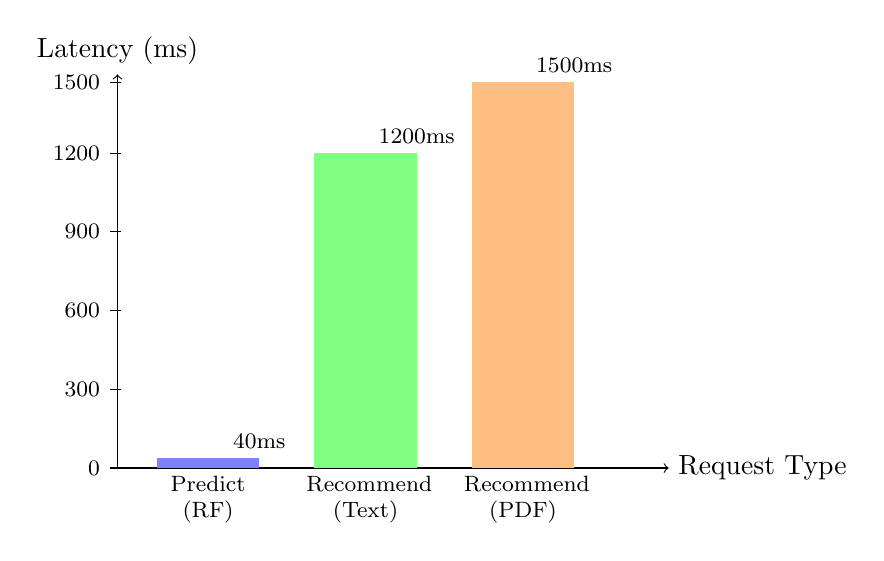
\begin{tikzpicture}
  \begin{scope}
    % Axes
    \draw[->] (0,0) -- (7,0) node[right] {Request Type};
    \draw[->] (0,0) -- (0,5) node[above] {Latency (ms)};

    % Y-axis labels
    \foreach \y/\label in {0/0, 1/300, 2/600, 3/900, 4/1200, 4.9/1500}
      \draw (0.05,\y) -- (-0.1,\y) node[left, font=\footnotesize] {\label};

    % Bars
    \fill[blue!50] (0.5,0) rectangle (1.8, 0.13) node[above, font=\footnotesize, black] {40ms};
    \fill[green!50] (2.5,0) rectangle (3.8, 4.0) node[above, font=\footnotesize, black] {1200ms};
    \fill[orange!50] (4.5,0) rectangle (5.8, 4.9) node[above, font=\footnotesize, black] {1500ms};

    % X-axis labels
    \node[font=\footnotesize, text width=1.5cm, align=center] at (1.15, -0.4) {Predict\\ (RF)};
    \node[font=\footnotesize, text width=1.5cm, align=center] at (3.15, -0.4) {Recommend\\ (Text)};
    \node[font=\footnotesize, text width=1.5cm, align=center] at (5.15, -0.4) {Recommend\\ (PDF)};
  \end{scope}
\end{tikzpicture}
\caption{API response latency comparison across endpoint types}
\label{fig:latency_bar}
\end{figure}

\section{Discussion}

\subsection{Dual-AI Complementarity}
The system's dual-AI approach proves highly effective. The local Random Forest model provides near-instantaneous, privacy-preserving disease classification from structured symptom inputs. The Groq LLM complements this by handling unstructured free-text inputs and semi-structured PDF clinical documents---a task the classical ML model is architecturally incapable of performing. Together, they cover a broad spectrum of real-world patient input modalities.

\subsection{API Deprecation Handling}
A significant practical challenge encountered during development was the upstream deprecation of Groq's \texttt{llama-3.2-11b-vision-preview} model. This model had been planned for processing raw image uploads (JPG/PNG). Its decommissioning required a rapid architectural pivot: the system was refactored to explicitly reject image uploads with a descriptive, user-friendly error message and to instead favor PDF text extraction via \texttt{PyPDF2}. This demonstrates the importance of building graceful degradation logic into AI-dependent systems, as external API surfaces are subject to change without warning.

\subsection{User Experience Refinements}
User testing feedback drove two significant UI improvements:
\begin{itemize}
    \item \textbf{Cancel Upload Button:} The initial file input provided no mechanism to deselect an uploaded file. A ``Remove'' button was added that clears the React state variable, replacing the file pill with the original file input field.
    \item \textbf{Two-Column Card Layout:} The original single-column form layout placed the file upload section far below the fold, making it easy to miss. Refactoring to a side-by-side two-card CSS Grid layout made both input options immediately visible and equally prominent.
\end{itemize}

\subsection{Limitations Observed in Practice}
\begin{itemize}
    \item \textbf{Scanned PDFs:} Patients who save screenshots of their reports as PDF files produce documents where all content is embedded as image data. \texttt{PyPDF2} cannot extract text from such files. The system correctly handles this by returning a descriptive error, but a future enhancement would involve integrating an OCR library (such as \texttt{pytesseract}) for scanned document support.
    \item \textbf{Groq Rate Limiting:} Under high usage, the Groq API may return HTTP 429 (Too Many Requests). The frontend implements a countdown timer to transparently inform the user of the retry window.
    \item \textbf{RF Model Coverage:} The Random Forest model is limited to the 41 disease classes and 132 symptoms defined in its training dataset. Rare or novel diseases outside this scope cannot be predicted.
\end{itemize}
